\subsection{Pianificazione del lavoro}

%stima iniziale
La pianificazione iniziale del lavoro prevedeva la distribuzione delle trecento ore nel modo seguente:
\begin{enumerate}
	\item	40 ore:     studio di Ruby on Rails, Drools e del software esistente;
	\item	50 ore:		analisi dei requisiti e dei miglioramenti da effettuare al codice esistente
	\item	40ore:		riprogettazione delle componenti esistenti che presentano criticità e delle nuove componenti
	\item	100 ore:     codifica di funzionalità e test;
	\item	40 ore:		implementazione delle regole Drools;
	\item 	15 ore:		 stesura della documentazione;
	\item	15 ore: 	verifica.
\end{enumerate}

%
%\begin{figure}[H]
%	\begin{center}
%		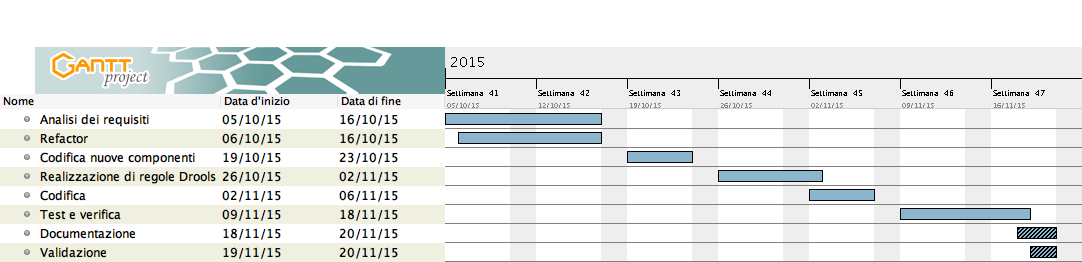
\includegraphics[width=16cm]{Pics/gantt.png}
%		\caption{Diagramma di Gantt.}
%		\label{fig:Gantt}
%	\end{center}
%\end{figure}
%


Durante lo stage, le ore sono state mantenute tali e quali alle previsioni. Tuttavia, la loro distribuzione nel tempo è leggermente cambiata rispetto al piano di lavoro. \\
L'attività di sviluppo è stata divisa in due parti distinte:  la prima relativa alla riprogettazione e codifica delle componenti già presenti al momento dell'inizio dello stage, la seconda relativa allo sviluppo delle nuove componenti.
A seguito di una riunione con il committente, si sono rese necessarie alcune modifiche che hanno provocato una leggera variazione del piano di lavoro.\\

Nello specifico l'ordine di esecuzione con le relative ore impiegate sono state le seguenti:
\begin{enumerate}
	\item	40 ore:     studio di Ruby on Rails, Drools e del software esistente;
	\item	20 ore:     rilevamento delle  criticità sulle componenti esistenti ;
	\item	30 ore:		analisi dei requisiti
	\item	15 ore:		riprogettazione delle componenti esistenti che presentano criticità
	\item	20 ore:     progettazione delle nuove entità richieste;
	\item	80 ore:     codifica di funzionalità e test;
	\item	4 ore:       colloquio con il committente per validare le nuove modifiche;
	\item 	4 ore:		 riprogettazione delle componenti da modificare;
	\item  	22 ore:	 	codifica di funzionalità e test;
	\item	40 ore:		implementazione delle regole Drools;
	\item 	15 ore:		 stesura della documentazione;
	\item	15 ore: 	verifica.
\end{enumerate}

Il conteggio totale delle ore al termine dello stage è di trecentocinque.
Data la complessità del progetto, le ore disponibili sono state sufficienti alla realizzazione delle funzionalità tali da soddisfare tutti i requisiti obbligatori e desiderabili, ma nessuno di quelli opzionali.